% ─────────────────────────────────────────────────────────────
% SPB: A Surplus-Preserving Bargaining Protocol for LLM Multi-Agent Negotiation
% Target: Applied Intelligence (Springer)
% Draft 2026-10-23. Internal draft uses the article class; convert to
% Springer Nature's sn-jnl class before submission.
% ─────────────────────────────────────────────────────────────
\documentclass[11pt]{article}

\usepackage[margin=2.4cm]{geometry}
\usepackage{amsmath,amssymb}
\usepackage{graphicx}
\usepackage{booktabs}
\usepackage{multirow}
\usepackage{float}
\usepackage{caption}
\usepackage{enumitem}
\usepackage{xcolor}
\usepackage[colorlinks=true,linkcolor=blue,citecolor=blue,urlcolor=blue]{hyperref}
\usepackage{array}

\title{\textbf{SPB: A Surplus-Preserving Bargaining Protocol\\ for LLM Multi-Agent Negotiation}}
\author{Wang Yinbing\thanks{School of Computer Science, Beijing Information Science and Technology University, Beijing, China.}}
\date{}

\setlength{\emergencystretch}{2.5em}
\begin{document}
\maketitle

\begin{abstract}
\noindent Large language model (LLM) agents agree easily. In 300 two-agent negotiations over a shrinking pie, both sides accepted the same split in 99.7\% of episodes, on average in round 2.1. Yet none of those agreements was executed: free dialogue contains no rule that pays the split out. The same transcripts score 0.39 or 0.90 depending on whether one credits the last mutual acceptance or the first one; reading only the final rounds misses 13 of the 300 agreements. Agreement is therefore not a deal. An execution rule is necessary, but its form decides the outcome: a strict hook closes 42\% (0.26), a forgiving one that accepts ordinary language 70\% (0.57), and neither approaches SPB's 1.000 in a single round. Structured protocols avoid the problem because execution is the default path: a sealed-demand rule with a proportional compromise (SPB) reaches 1.000 and 0.998 on two DeepSeek backbones, against 0.935 and 0.972 for a destructive sealed-bid baseline, in one round and at a fifth to a tenth of the free-dialogue token cost. The commitment check, assumed free, costs 4--13 efficiency points and inflates demands from 6.23 to 7.57; post-hoc self-reports recover 67\% of the agreements (76\% proposer, 97\% responder); and the value of the compromise is set by how often sealed demands are incompatible --- nil in GLM-4.5-Air, where they always clear (1.000 in both arms), and nil in Qwen3-32B, which rejects 29\% of compromises (0.757 against 0.752), with the confirmation step acting as the remedy there (0.979).
\end{abstract}

% ═══════════════════════════════════════════════════════════
\section{Introduction}

Multi-agent systems built from large language models (LLMs) are now used for software development~\cite{chatdev,metagpt}, optimisation modelling~\cite{dualtime}, tool use~\cite{autogen} and negotiation. In all of these settings the agents must agree on something: who does which subtask, which answer to submit, how to split a payoff. The rules that govern that agreement --- who speaks when, what may be said, what counts as consent, and what happens when the parties fail to converge --- constitute the \emph{communication protocol}.

Surveys of LLM-based multi-agent systems classify protocols~\cite{guo2024survey,chen2024survey,beyondselftalk} but do not measure them. Empirical work compares frameworks~\cite{maseval,mafbench}, agent counts~\cite{multi_llm_agent,scaling2026}, or topologies~\cite{gdesigner}, and typically reports task accuracy, success rate or cost. Very little work reports the quantity that a deployer actually cares about when the agents are negotiating over a scarce resource: \emph{how much of the resource is still there when the deal closes}. A protocol that closes 95\% of negotiations after the pie has shrunk by half is worse than one that closes 100\% immediately.

This paper makes four contributions.

\begin{enumerate}[leftmargin=*,itemsep=2pt]
\item \textbf{Agreement is not a deal.} We show that an execution event, not agreement, is what makes welfare measurable. The same 300 transcripts yield an efficiency of 0.39 or 0.90 depending on whether one credits the last mutual acceptance or the first; a reading restricted to the final four rounds misses 13 of 300 agreements. For free-form negotiation there is no execution event, so any welfare number presupposes a convention that is rarely stated.

\item \textbf{A protocol that executes.} We propose Surplus-Preserving Bargaining (SPB): simultaneous sealed demands, a proportional compromise when demands are incompatible, and an optional commitment check. SPB attains 1.000/0.998 against 0.935/0.972 for a destructive sealed-bid baseline, in a single round, at about a tenth of the tokens free dialogue consumes.

\item \textbf{Evidence that verification is not free.} The commitment-check variant lowers efficiency (0.871/0.960) and, in the smaller model, raises mean demand from 6.23 to 7.57. Adding confirmation to improve reliability is paid for in welfare.

\item \textbf{A measurement result.} The posterior self-report recovers 67\% of the agreements (76\% for the proposer, 97\% for the responder) where an adjudicated reading finds 95--100\%, and it is role-asymmetric: the agent that proposes counts the settlement as an agreement far less often than the agent that accepts.
\end{enumerate}

SPB builds on the sealed-bid bargaining rule of Chatterjee and Samuelson~\cite{chatterjee1983}; what we contribute is the empirical question of what happens when its no-trade branch is replaced by a compromise, and a measurement protocol that can answer that question without relying on the agents' own reports.

The remainder of the paper is organised as follows. Section~\ref{sec:related} reviews related work. Section~\ref{sec:problem} formalises the game and the protocols. Section~\ref{sec:spb} presents SPB. Section~\ref{sec:setup} describes the experimental design and the measurement instruments. Section~\ref{sec:results} reports results and Section~\ref{sec:discussion} discusses implications and limitations.

% ═══════════════════════════════════════════════════════════
\section{Related Work}
\label{sec:related}

\subsection{Frameworks and communication protocols}

AutoGen~\cite{autogen} provides group-chat primitives (\texttt{SelectorGroupChat}, \texttt{RoundRobinGroupChat}); MetaGPT~\cite{metagpt} and ChatDev~\cite{chatdev} encode role-based software teams; graph-based orchestration proposes learned topologies~\cite{gdesigner}. These systems embed a protocol, but the protocol is rarely the object of study. Recent surveys~\cite{beyondselftalk,protocoltax} note that coordination efficiency, bandwidth and latency are not captured by existing leaderboards. Our work isolates the protocol as the independent variable and measures its effect on welfare.

\subsection{When do multiple agents help?}

A growing 2026 literature compares multi-agent systems with single-agent baselines under controlled budgets. Tran and Kiela~\cite{equalbudget} report that single-agent systems outperform multi-agent systems on multi-hop reasoning once thinking-token budgets are equalised. BenchAgent~\cite{benchagent} compares six multi-agent workflows with a single-agent reference across ten benchmarks and finds that five of the six trail the reference, some while consuming 4.3$\times$ the tokens. Other work reaches similar conclusions at equal inference cost~\cite{equalinference}, for skill-based single agents~\cite{skillsreplace}, and in user-facing dual-control settings~\cite{dualcontrol}. Theoretical accounts of when coordination helps are beginning to appear~\cite{taxmodel,infobottleneck}.

Our question is different and complementary. We do not ask whether to use multiple agents; we ask, given that agents must negotiate, which protocol leaves the least value on the table. The two questions share a commitment to explicit baselines and cost accounting.

\subsection{LLM agents in strategic settings}

LLMs have been evaluated as players in prisoner's dilemma, ultimatum and public-goods games~\cite{llm_cooperate,gamebench}; they tend to cooperate at least as much as humans. Closest to our work, Albayaydh and Zhao~\cite{mechanism2026} encode alternating-offers bargaining and auctions as constraints over A2A/MCP message schemas~\cite{a2a}, add a runtime verification layer, and report that structured protocols achieve 100\% success while a three-party fair-allocation task yields only 4.2\% usable outcomes. We differ in three respects: we measure \emph{welfare} rather than success, we propose a compromise rule that eliminates discard, and we treat the measurement instrument itself as an object of study.

\subsection{Mechanism design and bargaining theory}

Rubinstein~\cite{rubinstein1982} shows that in alternating offers with discounting the equilibrium split depends on the discount factor and the order of play; Nash~\cite{nash1950} axiomatises the symmetric bargaining solution; Myerson~\cite{myerson1991} formalises mechanism design. These results assume optimising players. LLM agents are not optimisers: they reason in language, carry cooperative priors from alignment training~\cite{llm_cooperate}, and are sensitive to framing. Our protocols are therefore evaluated behaviourally, with the classical results used as benchmarks rather than as predictions.

The closest classical antecedent to our mechanism is the sealed-bid bargaining rule of Chatterjee and Samuelson~\cite{chatterjee1983}: both parties submit simultaneous private bids, trade occurs if the bids are compatible, and otherwise there is no trade. SPB keeps the sealed-demand stage and replaces the no-trade outcome with a proportional compromise. This replacement matters because Myerson and Satterthwaite~\cite{myerson1983} show that with two-sided private information no mechanism can be simultaneously efficient, incentive compatible, individually rational and budget balanced. SPB gives up incentive compatibility to recover efficiency in the incompatible branch, and Section~\ref{sec:demand} measures the price of that trade-off: demand inflation.

% ═══════════════════════════════════════════════════════════
\section{Problem Setting}
\label{sec:problem}

\subsection{The bargaining game}

Two agents, $A$ and $B$, negotiate over a pie that shrinks over time. There are at most $T$ rounds. The pie in round $r$ is
\begin{equation}
P_r = \max\left(1,\ \mathrm{round}\left(R\,\delta^{r-1}\right)\right), \qquad \delta=0.9,\ R=10,
\end{equation}
so $P_1=10$ and $P_{10}=4$. If the agents agree in round $r$ on shares $(x_A,x_B)$ with $x_A+x_B\le P_r$, those shares are paid and any unallocated remainder is lost. If no agreement is reached by round $T$, both receive zero. Each agent maximises its own payoff and is told not to care about the other's.

The discount is not cosmetic: it makes delay costly in the payoff itself, so that ``agreeing late'' and ``agreeing on a bad split'' are both visible in the same currency.

\subsection{Protocols as mechanisms}

A protocol is a tuple $\mathcal{M}=(S,\pi,\tau)$: a message space $S$, an allocation rule $\pi$, and a round structure $\tau$ (who moves when, and what is observed). We study five protocols:
\begin{itemize}[leftmargin=*,itemsep=1pt]
\item \textbf{Free dialogue}: unconstrained natural language, no termination rule, no commitment device.
\item \textbf{Alternating offers}: Rubinstein-style; the proposer states a split, the responder accepts or rejects, and the right to propose alternates.
\item \textbf{Sealed bid}: both agents privately state a demand; compatible demands ($d_A+d_B\le P_r$) are executed, incompatible rounds yield nothing and the pie shrinks.
\item \textbf{SPB} (ours): sealed demands plus a proportional compromise when demands are incompatible.
\item \textbf{SPB+} (ours): SPB plus a commitment check that voids unconfirmed deals.
\end{itemize}

\subsection{Allocative efficiency}
\label{sec:eff}

For an episode with initial pie $R$, let $e\in\{0,1\}$ indicate whether a deal was \emph{executed} --- that is, whether the protocol's rule actually paid a split out --- and let $A_{\text{alloc}}$ be the total allocated. We define
\begin{equation}
\mathrm{Eff} = \frac{e\cdot A_{\text{alloc}}}{R}\in[0,1].
\label{eq:eff}
\end{equation}
Efficiency decomposes into two losses: \emph{discard} (a deal is struck but $A_{\text{alloc}}<P_r$) and \emph{delay} ($P_r<R$ because the deal was late). The two are exchangeable in this metric: a deal in round 9 for 4 of 10 points and a deal in round 1 for 6 of 10 both score 0.4.

The definition hinges on $e$. Structured protocols supply an execution event --- a compatible sealed bid, an accepted offer, a confirmed compromise --- and the rule, not the analyst, decides that a deal happened. Free dialogue supplies no such event: an agreement there is a fact about the transcript, not about the system. We therefore report free-dialogue welfare under three explicit conventions (Section~\ref{sec:measure}) rather than one, and argue that any study of free-form negotiation has to state which convention it uses.

\section{The SPB Protocol}
\label{sec:spb}

SPB has three components; the first is shared with the sealed-bid baseline, the other two are new.

\paragraph{(1) Sealed demand.} Each round, each agent privately submits an integer demand $d_i\in[0,P_r]$ in a machine-readable format. Neither agent observes the other's demand. If $d_A+d_B\le P_r$ the deal executes at $(d_A,d_B)$, and any unclaimed remainder is lost.

\paragraph{(2) Proportional compromise.} If $d_A+d_B>P_r$, the mechanism does not discard the pie. It proposes the proportional split
\begin{equation}
x_A=\mathrm{round}\!\left(\frac{d_A}{d_A+d_B}P_r\right),\qquad x_B=P_r-x_A,
\end{equation}
and each agent replies ACCEPT or REJECT. If both accept, the deal executes; otherwise the next round begins on a smaller pie.

\paragraph{(3) Commitment check (SPB+ only).} Whenever a deal is proposed --- at the demanded split or at the compromise split --- both agents must reply CONFIRM. If either refuses or fails to confirm, the deal is void and the round is lost.

\paragraph{Design rationale.} The compromise rule converts an incompatible round from a total loss into a proportional one, so the mechanism is surplus-preserving by construction: every round in which at least one agent accepts ends with the whole pie allocated. The rule is deliberately \emph{proportional} rather than equal. Under an equal-split fallback, compatible demands would still execute as demanded, but the fallback payoff would no longer depend on how much either agent asked for; the demand stage would become a coordination problem (find any compatible pair) rather than an extraction problem, and the experiment could not reveal whether a mechanism induces demand inflation. Proportional division keeps the demand informative in both branches, which is what makes the demand-inflation result measurable. The commitment check is included as a separate component precisely because verification is often assumed to be free; our ablation tests that assumption.

% ═══════════════════════════════════════════════════════════
\section{Experimental Setup}
\label{sec:setup}

\subsection{Models}

We use two backbones from one family, served through the same OpenAI-compatible endpoint: \texttt{deepseek-flash} (DeepSeek-V4.1-Flash, the smaller tier) and \texttt{deepseek-v4-pro} (DeepSeek-V4-Pro, the larger tier). Both are pinned to \texttt{reasoning\_effort=none}: in their default configuration both models spend the entire output budget on hidden reasoning and return empty content for short decision turns, which makes per-turn cost incomparable. Temperature is 0.3 throughout.

\subsection{Design}

Five protocols $\times$ two models $\times$ 30 trials $\times$ 5 repeated episodes $=$ 1{,}500 episodes. Within a trial, the same pair of agents plays five episodes in sequence and is shown only the \emph{outcomes} of previous episodes (who received what), not the transcripts. This isolates learning-from-outcome from context-length effects. Agents keep their roles (A always moves first in alternating offers) across episodes.

All prompts are in English and identical across protocols except for the protocol rules. Round limits: $T=10$ for all protocols. The full prompt set, the raw transcripts, and the analysis scripts are released with the paper.

\subsection{Measurement instruments}

The outcome of a negotiation can be read in several ways; we report four.

\begin{enumerate}[leftmargin=*,itemsep=2pt]
\item \textbf{Mechanism outcome} (structured protocols). The protocol's own rule decides: compatible demands, an accepted offer, or a deal confirmed by both parties.
\item \textbf{Adjudicated transcript reading} (free dialogue only). A transcript adjudicator (DeepSeek-V4-Pro, temperature 0) reads the \emph{whole} transcript and reports the first round in which both agents accept the same split, together with the split. A second variant, which reads only the final four rounds, is retained as a diagnostic: it is the convention used in an earlier version of this study, and the gap between the two is itself a result (Section~\ref{sec:measure}). We hand-coded 20 episodes against the full transcript --- the 13 in which the two variants disagreed, the single no-deal episode, and six of the remaining agreements drawn at random. The adjudicator matched the hand reading in 19; the one miss placed a first agreement at round~5 instead of round~2 in an episode where the accepting agent restated its deliberation before accepting at the end.
\item \textbf{Strict symmetric detector} (diagnostic). A deterministic rule that certifies a deal only if, in the same round, \emph{both} agents use an explicit acceptance token and \emph{both} name the same symmetric split. We report it to show how a conservative rule behaves; it is not the primary measure.
\item \textbf{Post-hoc self-report}. At the end of each episode each agent is asked, with an identical prompt, whether the two agents agreed on a split and, if so, what it was. A deal counts only if both agents say YES and report the same split.
\end{enumerate}

We additionally apply the regex parser from an earlier pilot study of ours (released as \texttt{legacy\_parser.py}) to the free-dialogue transcripts, to quantify how much of a headline number can be produced by the instrument alone.

\subsection{Metrics and statistics}

Per episode we record: deal indicator, allocated amount, efficiency, rounds to agreement, mean demand, whether a compromise was offered and accepted, whether confirmation failed, and API-reported token usage. We report means, Wilson 95\% intervals for proportions, and bootstrap 95\% intervals (3{,}000 resamples) for the key efficiency comparisons. Protocol effects are tested with Kruskal--Wallis across the five protocols and with pairwise Mann--Whitney tests; learning is tested with a per-protocol linear slope of efficiency on episode index.

% ═══════════════════════════════════════════════════════════
\section{Results}
\label{sec:results}

\subsection{Agreement is universal; execution is not}

Table~\ref{tab:main} and Fig.~\ref{fig:main} report the main results. Agreement is almost universal: sealed bidding and SPB close essentially every negotiation, and even free dialogue produces a mutually accepted split in 99\% of episodes, in round 3.3 (flash) and round 1.0 (pro). Execution is what separates the protocols. A sealed bid executes when the demands are compatible and SPB when the compromise is accepted; free dialogue has no rule that turns an agreement into a transaction, so its executed volume is zero by construction. Under the efficiency definition of Section~\ref{sec:eff}, the free-dialogue arm therefore scores zero no matter how cooperative the agents are.

\begin{table}[H]
\centering
\caption{Main results. ``Agreed'' is the share of episodes in which both agents accepted the same split of the same pie; ``Executed'' is the share in which the protocol's rule actually paid a split out. Efficiency is executed allocation over the initial pie $R=10$. For free dialogue, rounds is the adjudicated round of the first mutual acceptance. Tokens are mean API-reported tokens (input + output) per episode.}
\label{tab:main}
\small\setlength{\tabcolsep}{4pt}
\begin{tabular}{@{}llcccccc@{}}
\toprule
Model & Protocol & $n$ & Agreed & Executed & Efficiency & Rounds & Tokens \\
\midrule
\multirow{5}{*}{flash}
 & Free dialogue        & 150 & 0.99 & 0.00 & 0.000 & 3.3 & 52{,}559 \\
 & Alternating offers   & 150 & 0.87 & 0.87 & 0.805 & 1.8 &  7{,}805 \\
 & Sealed bid           & 150 & 1.00 & 1.00 & 0.935 & 1.6 &  4{,}206 \\
 & SPB (ours)           & 150 & 1.00 & 1.00 & \textbf{1.000} & 1.0 &  4{,}558 \\
 & SPB+ (ours)          & 150 & 0.93 & 0.93 & 0.871 & 1.8 & 14{,}487 \\
\midrule
\multirow{5}{*}{pro}
 & Free dialogue        & 150 & 1.00 & 0.00 & 0.000 & 1.0 & 19{,}310 \\
 & Alternating offers   & 150 & 1.00 & 1.00 & 0.865 & 2.9 &  5{,}892 \\
 & Sealed bid           & 150 & 0.99 & 0.99 & 0.972 & 1.2 &  3{,}588 \\
 & SPB (ours)           & 150 & 1.00 & 1.00 & \textbf{0.998} & 1.0 &  3{,}906 \\
 & SPB+ (ours)          & 150 & 1.00 & 1.00 & 0.960 & 1.4 &  5{,}043 \\
\bottomrule
\end{tabular}
\end{table}


\begin{figure}[H]
\centering
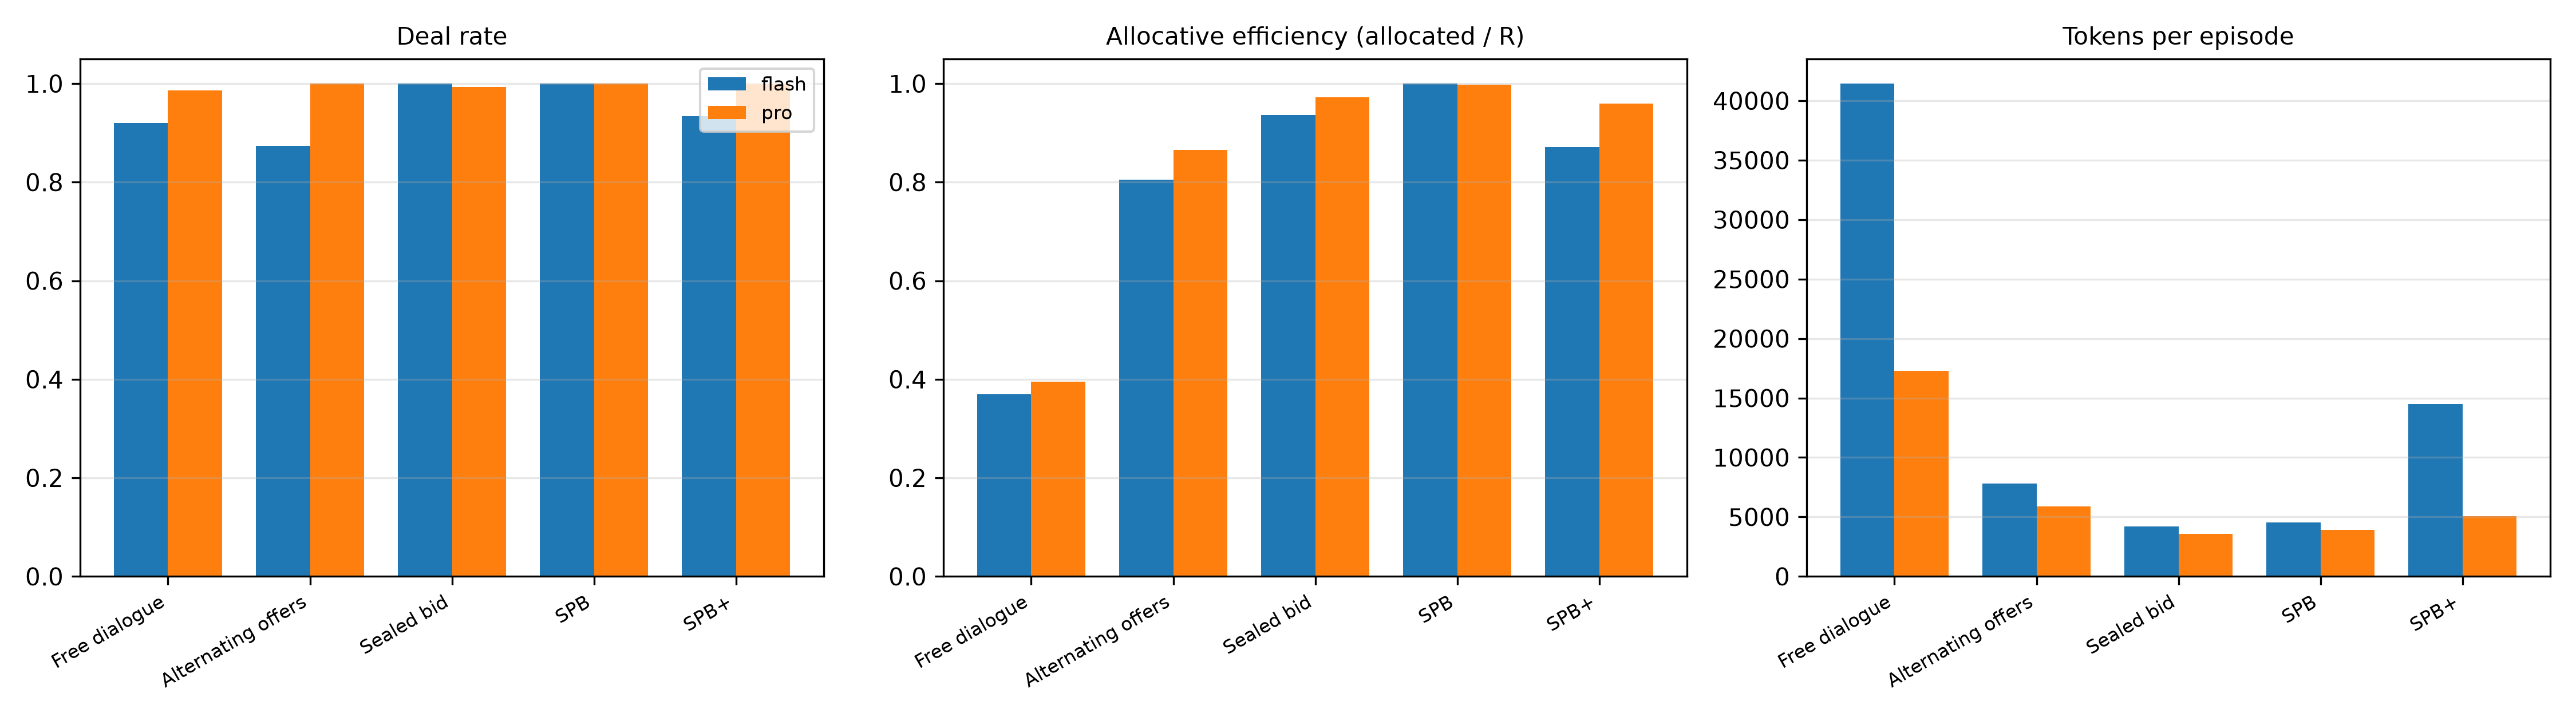
\includegraphics[width=\textwidth]{output_v3/main/analysis/fig1_main.png}
\caption{Agreement, executed efficiency and token cost by protocol and model. Agreement is high almost everywhere; execution is not. Free dialogue agrees in most episodes but executes nothing --- its executed column is zero by construction, because the protocol contains no rule that pays a split out --- and it costs 5--11 times as many tokens as SPB.}
\label{fig:main}
\end{figure}

Among the protocols that do execute, the effect is large and statistically reliable: Kruskal--Wallis across the five protocols gives $H=325.9$ ($p=2.8\times10^{-69}$) for flash and $H=465.4$ ($p=2.0\times10^{-99}$) for pro. The two-way comparison that motivates SPB is significant in both models: SPB vs.\ sealed bid, $p=3.9\times10^{-18}$ (flash) and $p=2.1\times10^{-4}$ (pro). All ten pairwise comparisons per model are Holm-corrected; both of these survive (adjusted $p=2.0\times10^{-17}$ and $6.2\times10^{-4}$). In the smaller model the gap is 6.5 efficiency points; in the larger model it is 2.6 points, because the larger model already bids close to the fair share.

Free dialogue is also the most expensive arm. It consumes 52{,}559 tokens per episode in flash and 19{,}310 in pro --- 11 and 5 times the SPB cost --- to produce an agreement that the system never acts on. A protocol that agrees cheaply and executes is worth more than one that agrees expensively and does not.

\paragraph{The discount factor is not doing the work.}
Efficiency depends on $\delta$ through the value of a round, so we recomputed it from the same episodes at $\delta=0.80$ and $\delta=0.95$, holding behaviour fixed. The ordering is unchanged: SPB 0.998 / 0.999 / 1.000, sealed bid 0.912 / 0.954 / 0.980, alternating offers 0.768 / 0.835 / 0.889, free dialogue under the first-agreement convention 0.838 / 0.905 / 0.946. Slower decay flatters every protocol and closes the gap between them, but it never reorders them.

\paragraph{Benchmark check: does a model play the Rubinstein equilibrium?}
With a per-round discount $\delta=0.9$, the subgame-perfect equilibrium of alternating offers gives the proposer the share $1/(1+\delta)=0.526$ of the current pie. In the 281 alternating-offer episodes that closed, the proposer's share is 0.509 for \texttt{pro} ($n=150$) and 0.624 for \texttt{flash} ($n=131$). The larger model sits within 1.7 percentage points of the benchmark, although the deviation is statistically detectable at this sample size ($t=-3.93$, $p=1.3\times10^{-4}$); the smaller model over-extracts by almost ten points ($t=10.8$, $p<10^{-19}$). The smaller model's deviation is asymmetric: A takes 0.558 when it proposes and B takes 0.673 when it does, which is a last-proposer advantage rather than equilibrium play. Because our protocol approximates Rubinstein (integer splits, finite horizon, rejection ends the round), we read these as deviations from a benchmark rather than as a test of equilibrium play. They connect the welfare result to behaviour: the protocol does not merely change when the pie is divided; it changes how far the division departs from the theoretical benchmark.

\subsection{The compromise is what preserves the surplus}

SPB's advantage is produced by the fallback, not by the sealed-demand stage, which it shares with the baseline. In the smaller model the compromise was offered in 83\% of episodes; in the larger model, 21\%. The interpretation is direct: the smaller model systematically over-demands ($\bar d_A=6.23$ vs.\ the fair share of 5), so its demands are usually incompatible; the compromise rule then rescues the round instead of discarding it. The larger model demands close to the fair share ($\bar d_A=5.20$), so the mechanism is needed less often.

SPB is also fast: 1.0 rounds in both models, against 1.2--1.6 for sealed bidding and 1.8--2.9 for alternating offers. Because the pie shrinks 10\% per round, this speed is worth real points, and it is the main reason SPB reaches full efficiency.

One caveat must be stated plainly: SPB's efficiency of 1.000 is a property of the rule, not a discovery about the models. Whenever the demands are incompatible the compromise allocates the entire pie, so conditional on acceptance the mechanism cannot fail to allocate. What the experiment measures is therefore upstream of that: whether agents accept the compromise at all (100\% of episodes in DeepSeek and GLM, 73\% in Qwen), what the rule costs in incentives (demands rise by 1.34 points, Section~\ref{sec:demand}), and what it costs in tokens. A mechanism that cannot fail to allocate is only useful if agents agree to use it, and on the models we test they do.

\subsection{Commitment checking is not free}

The ablation in Table~\ref{tab:main} contradicts the common assumption that verification is a free add-on. Adding the commitment check (SPB+) lowers efficiency from 1.000 to 0.871 in flash ($p=3.7\times10^{-10}$) and from 0.998 to 0.960 in pro ($p=8.1\times10^{-8}$). The mechanism is visible in the behaviour: mean demand rises from 6.23 to 7.57 in flash, the compromise is triggered in 97\% of episodes, and 2.7\% of episodes contain at least one failed confirmation. An extra confirmation round is a round in which the pie shrinks, and agents that anticipate a second chance demand more.

This is a design warning rather than a failure: a verification layer buys auditability, but it should be budgeted for, and it can be counter-productive when the pie is time-sensitive.

\subsection{Repeated play does not close the gap}

Fig.~\ref{fig:learning} shows executed efficiency across the five repeated episodes of a trial. Most protocols are flat, which is the point: the ordering is present from the first episode and repeated play does not close it. The two exceptions are alternating offers in the larger model (slope $+0.123$ per episode, $p<0.001$, $R^2=0.54$) and SPB+ in the smaller model ($+0.082$, $p<0.001$, $R^2=0.17$), both of which start low and climb. Sealed bidding drifts up slightly ($+0.036$ in flash, $+0.028$ in pro, both $p<0.001$, $R^2\le0.35$). SPB is at the ceiling in episode~1, so its slope is zero by construction. Free dialogue is excluded here: its executed efficiency is zero in every episode, so a slope is undefined.

\begin{figure}[H]
\centering
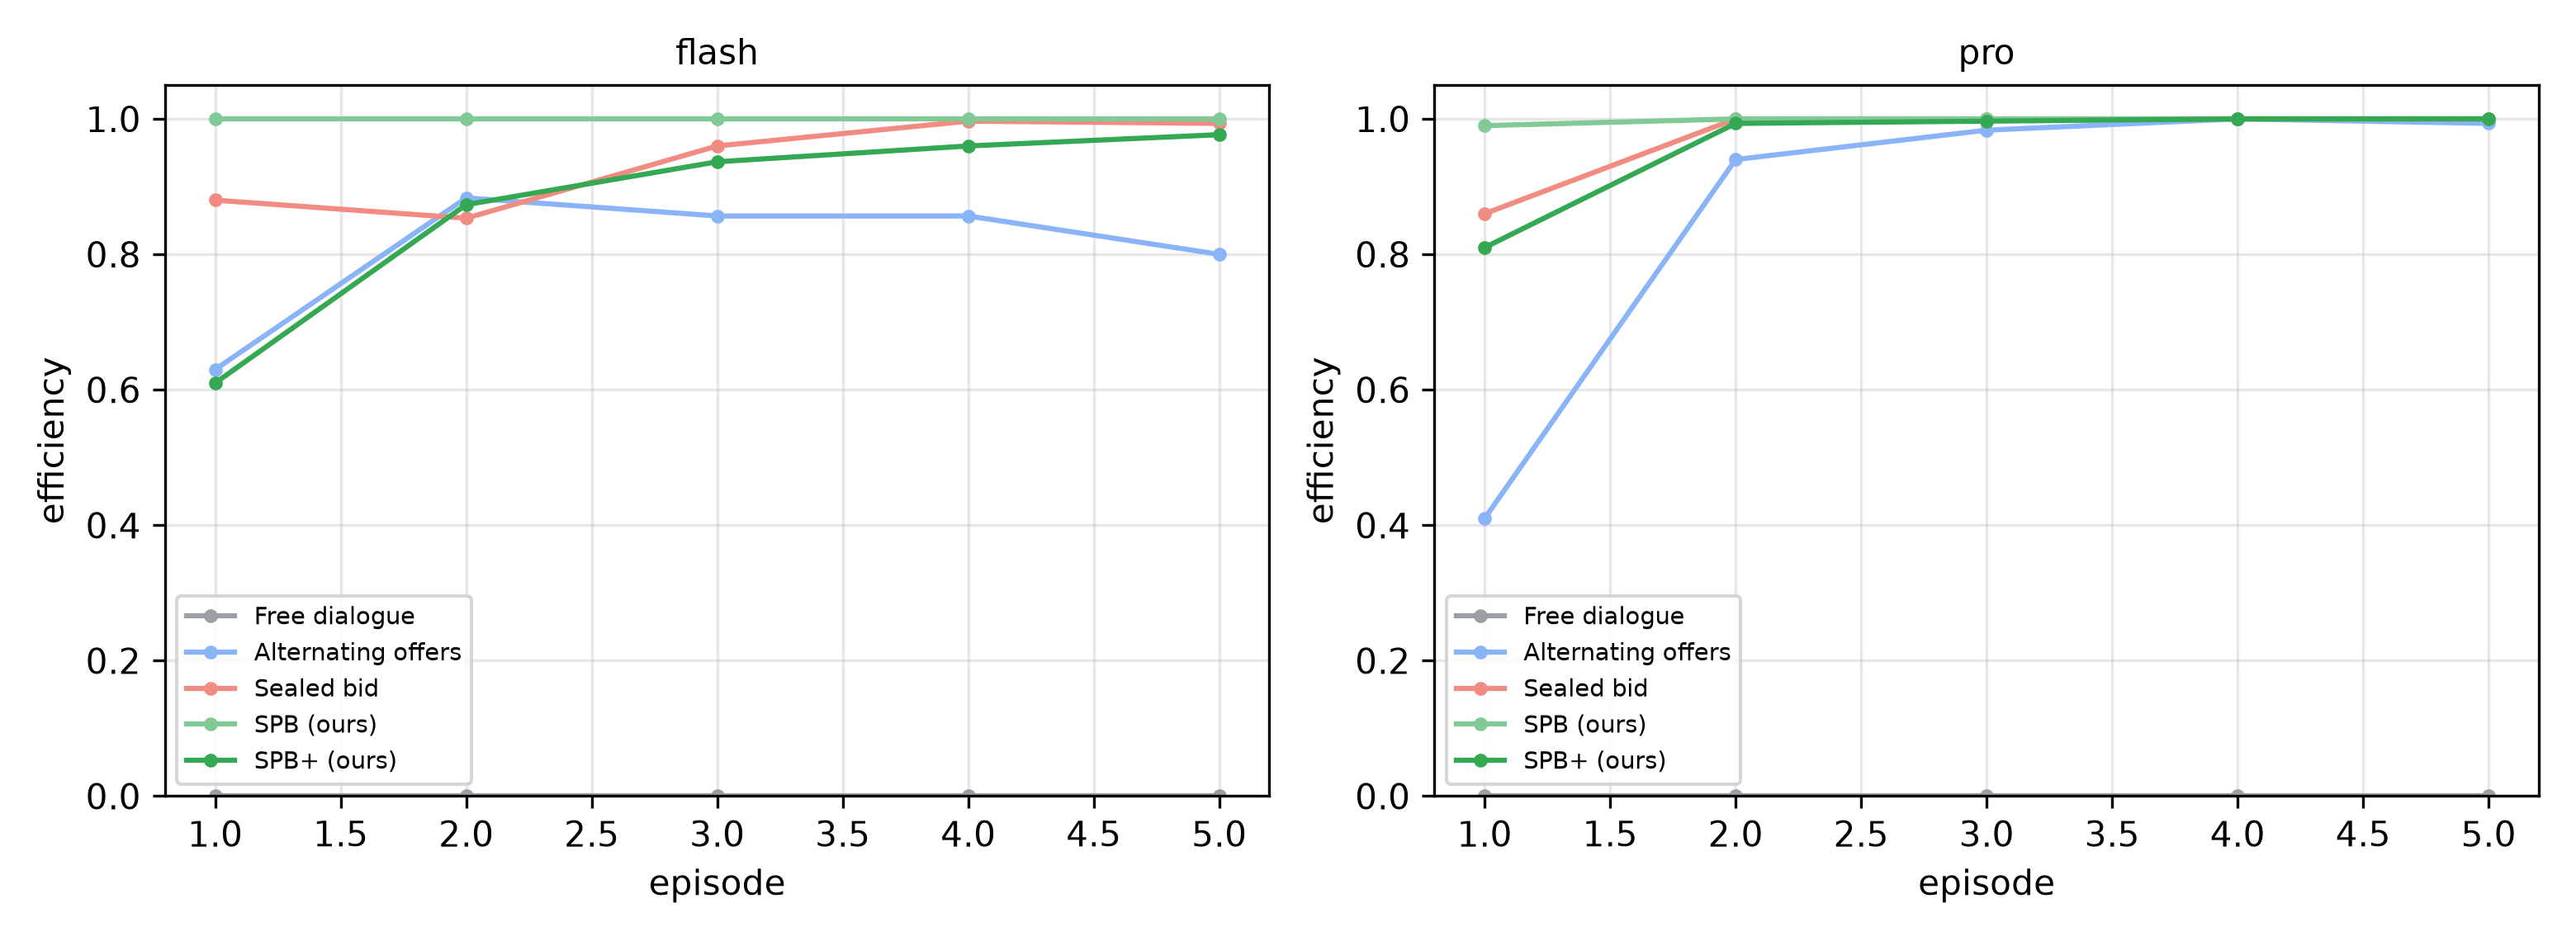
\includegraphics[width=\textwidth]{output_v3/main/analysis/fig2_learning.png}
\caption{Executed efficiency by repeated episode within a trial. SPB is at the ceiling from episode~1; alternating offers improve with repetition, steeply in the larger model; free dialogue executes nothing, so its curve is flat at zero.}
\label{fig:learning}
\end{figure}

The asymmetry is informative. Alternating offers give the agents a clear signal (accept/reject) attached to a specific proposal, and repetition lets them calibrate. Free dialogue gives no such signal: an agent cannot tell whether a concession was reciprocated or ignored, and the transcript grows rather than the policy improving.

\subsection{Demand inflation}
\label{sec:demand}

Fig.~\ref{fig:demand} plots the mean demand of Agent~A. In flash, the ordering is sealed (5.03) $<$ SPB (6.23) $<$ SPB+ (7.57). The proportional compromise rewards a higher demand with a higher share when demands are incompatible, so agents drift upward; the commitment check accelerates the drift. In pro the effect is much weaker (4.97, 5.20, 5.06), consistent with the larger model anchoring on the fair share. Demand inflation is the price SPB pays for surplus preservation, and it is the natural next target for mechanism design.

\textbf{Is the drift caused by the rule?} To separate the mechanism from the models we ran a third arm in which the fallback ignores the demands entirely: on incompatible demands the pie is split equally, so a higher demand buys nothing. If the drift were a response to the proportional reward, demands should return to the fair share. They do not. Mean demand of Agent~A is 5.90 against 6.23 in flash ($p=0.10$) and 5.09 against 5.20 in pro ($p=0.006$, a tenth of a point), and efficiency is unchanged (0.996 against 1.000, $p=0.32$; 1.000 against 0.998, $p=0.16$). Most of the over-demanding is therefore a property of the models rather than of the rule: these agents bid above the fair share even when bidding high cannot help them. The practical consequence is that removing the incentive is not enough to remove the behaviour, and an audit of demands should be part of deployment rather than a fix inside the mechanism.

\begin{figure}[H]
\centering
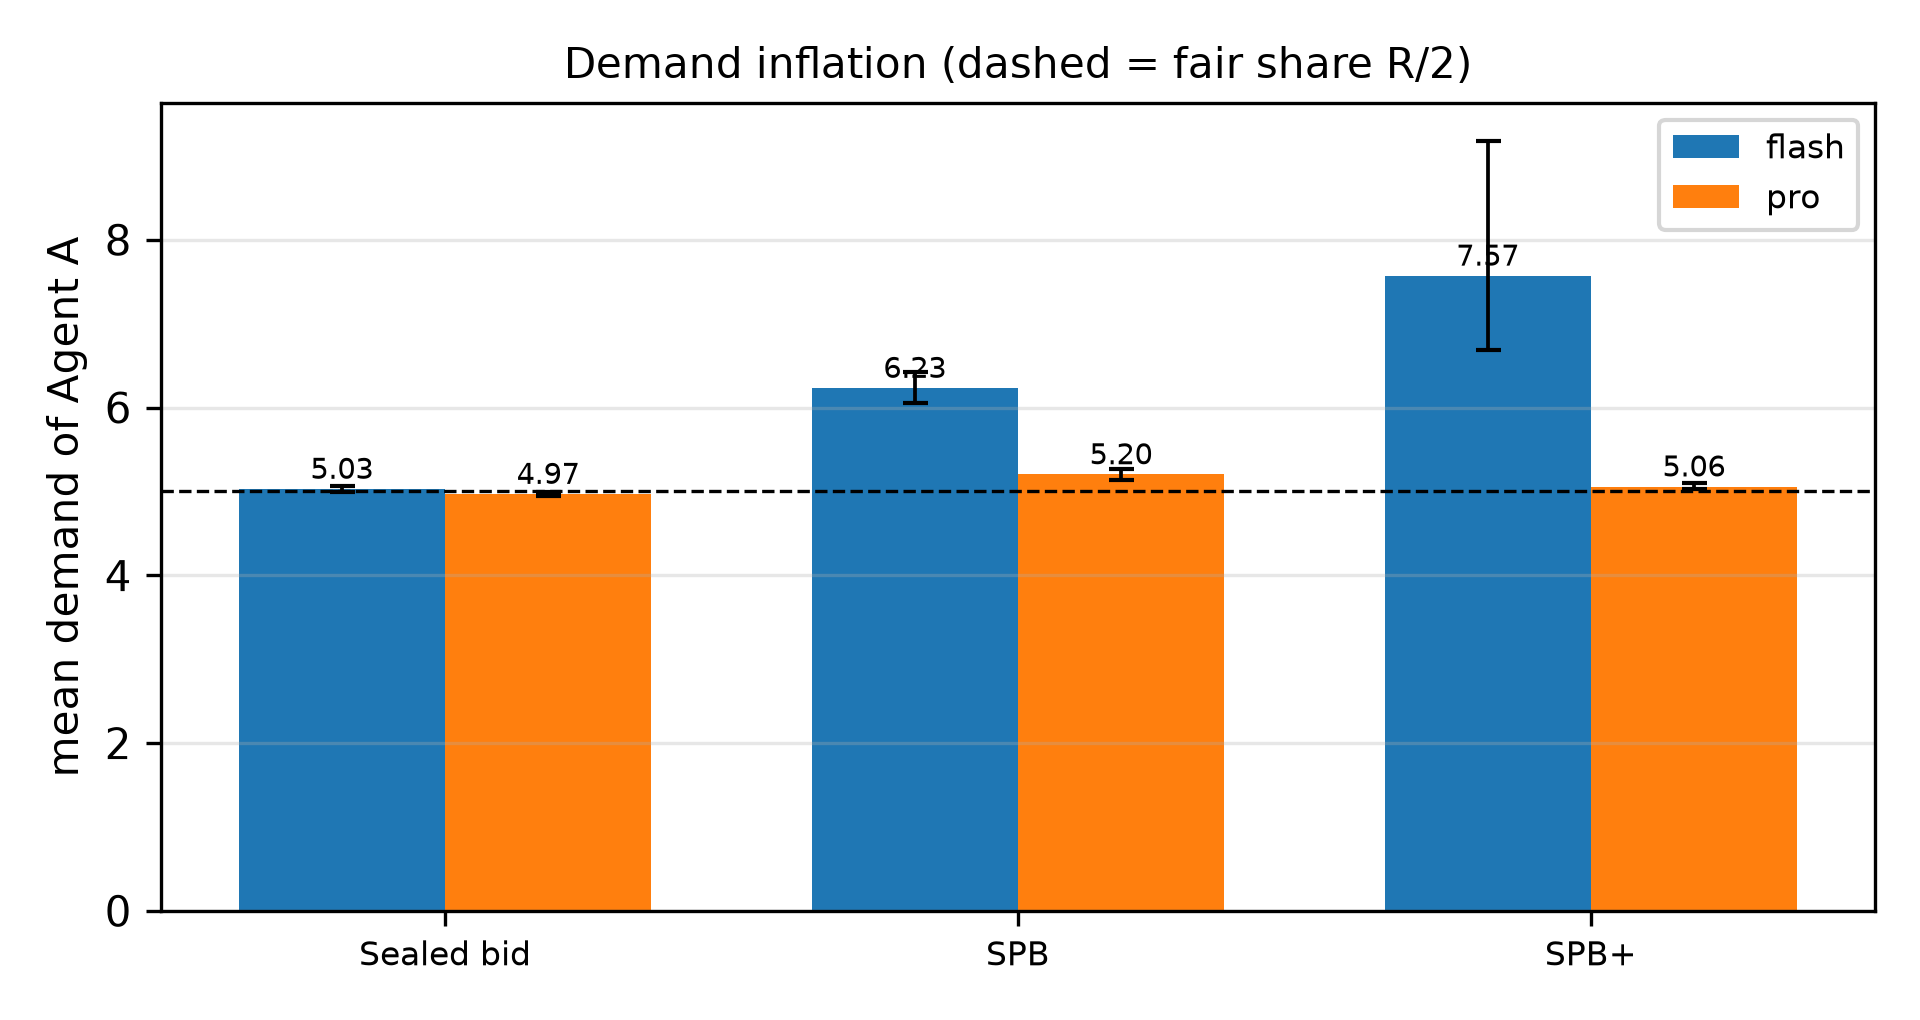
\includegraphics[width=0.62\textwidth]{output_v3/main/analysis/fig3_demands.png}
\caption{Mean demand of Agent~A by protocol and model. The dashed line is the fair share $R/2$. The compromise rule induces upward drift in the smaller model.}
\label{fig:demand}
\end{figure}

\subsection{Three readings, three answers}
\label{sec:measure}

Because free dialogue has no execution event, its welfare is not a property of the conversation alone: it depends on what the analyst counts as a deal. We report three operational readings: two conventions applied to the same 300 transcripts, and one separate arm in which the protocol does supply an execution rule.

\begin{table}[H]
\centering
\caption{Free dialogue under four operational readings. The first two apply different conventions to the same 300 transcripts; the last two are separate 300-episode arms with an execution rule, differing only in how strictly the closing move is encoded.}
\label{tab:conventions}
\small
\begin{tabular}{@{}lccc@{}}
\toprule
Convention & Deal rate & Mean round & Efficiency \\
\midrule
First mutual acceptance (convention)   & 0.997 & 2.1 & 0.905 \\
Last mutual acceptance (convention)    & 0.95  & 9.8 & 0.388 \\
Strict execution hook (formal syntax)  & 0.42  & 6.3 & 0.262 \\
Forgiving execution hook (free text)   & 0.70  & 3.4 & 0.567 \\
\bottomrule
\end{tabular}
\end{table}

The two acceptance conventions differ by a factor of 2.3, and the difference is structural rather than statistical. In free dialogue an agreement is typically reached early --- in 72\% of episodes in round 1 --- and the agents then keep restating it until the round limit, because nothing in the protocol stops them. A reading restricted to the final four rounds sees only the restatement: it places the deal at round 9.8 instead of 2.1, and it misses 13 of the 300 agreements outright, because in those episodes the closing rounds contain only ``Confirmed.'' and ``Done.'' and no split at all.

The posterior self-report fails in a different way, and the failure is role-asymmetric. Overall it recovers 67\% of the agreements, but the two roles disagree sharply: Agent~A, who proposes in every round, reports an agreement in 76\% of episodes, while Agent~B, who accepts, reports one in 97\%. The question asks whether \emph{both} agents stated acceptance of the same split; the proposer never ``accepts'' anything, so it answers no. A question that requires both parties to certify the same event does not measure a shared belief --- it measures the asymmetry of the roles.

The regex parser used in an earlier pilot recovers 91.7\% of the agreements at a mean round of 1.76, against 2.1 for the first-acceptance reference; it matches the reference round exactly in 57\% of episodes and within one round in 71\%. It is therefore a crude but not a biased instrument \emph{for the first agreement} --- but it certifies any early exchange that contains an acceptance word and a number pair, so it also credits proposals that were never accepted. Our deterministic strict detector, which requires an explicit symmetric acceptance in the same round, certifies 69.0\%: conservative by construction, and reported here to make the sensitivity of any conclusion to the reading rule visible.

The practical lesson is not ``use a better parser''. It is that the instrument defines the phenomenon. A study that credits the last acceptance reports 0.39 for a protocol that, on its own transcripts, achieves 0.91; a study that reads only the final rounds loses 4\% of the agreements entirely; and a study that asks the agents recovers two thirds of them, unevenly across roles. None of these numbers is wrong as arithmetic. They are answering different questions, and only one of them is about the system.

A strict reading would assign free dialogue an executed efficiency of zero, because the protocol was defined without any rule that pays a split out. Two arms test what an execution rule buys. In the first, a formal line is binding: \texttt{PROPOSE: A=<int>, B=<int>} states a split, \texttt{ACCEPT: A=<int>, B=<int>} accepts the other agent's most recent proposal, and a matching \texttt{ACCEPT} executes immediately and ends the episode. Every episode used the formal syntax at least once, so the shortfall is not one of compliance. It closes only 42\% of episodes, at round 6.3, for an efficiency of 0.262.

The second arm relaxes the encoding: ordinary language counts, so ``I accept 5-5'' executes the pending proposal. Closing rises to 70\%, the mean round falls to 3.4, and efficiency reaches 0.567 --- more than twice the strict arm. The form of the closing rule, not the willingness of the agents, is what moves the number.

Neither arm reaches SPB's 1.000 in a single round. The remaining gap is mechanical: in free dialogue the agents must first converge on a split and then encode it, and they anchor on stale splits as the pie shrinks; in SPB an incompatible demand triggers the compromise automatically and the deal executes without either agent deciding to stop. The gap is also model-dependent: under the forgiving hook the smaller model closes 94\% of episodes (efficiency 0.78) while the larger closes 45\% (0.35), which is the opposite ordering to the strict arm. Free dialogue also costs 13{,}800 tokens per episode against 4{,}500 for SPB.

\subsection{Cross-vendor replication}
\label{sec:crossvendor}

To test whether the protocol ranking survives a change of model family, we repeated the three sealed-demand protocols on two vendors served through a second API: Qwen3-32B (Alibaba) and GLM-4.5-Air (Zhipu). Prompts, game rules and measurement code are identical to the main experiment. Each cell contains 19--24 trials $\times$ 5 episodes, giving 110--150 episodes per cell (three episodes failed on rate limits and are excluded) (Table~\ref{tab:replication}).

\begin{table}[H]
\centering
\caption{Cross-vendor replication. Same prompts and measurement code as the main experiment; $n$ is the number of episodes per cell.}
\label{tab:replication}
\small
\begin{tabular}{@{}llccccc@{}}
\toprule
Model & Protocol & $n$ & Deal rate & Efficiency & Rounds & Tokens \\
\midrule
\multirow{3}{*}{GLM-4.5-Air}
 & Sealed bid & 110 & 1.00 & \textbf{1.000} & 1.0 & 3{,}369 \\
 & SPB (ours) & 118 & 1.00 & \textbf{1.000} & 1.0 & 5{,}117 \\
 & SPB+ (ours) & 113 & 0.96 & 0.933 & 1.3 & 7{,}970 \\
\midrule
\multirow{3}{*}{Qwen3-32B}
 & Sealed bid & 150 & 0.86 & 0.757 & 2.6 & 7{,}235 \\
 & SPB (ours) & 149 & 0.75 & 0.752 & 1.0 & 13{,}850 \\
 & SPB+ (ours) & 150 & 0.98 & \textbf{0.979} & 1.0 & 5{,}233 \\
\bottomrule
\end{tabular}
\end{table}

The two vendors pull the mechanism in opposite directions, and the reason is visible in the baseline. In GLM-4.5-Air the sealed demands are compatible in every one of 110 episodes, so sealed bidding already attains 1.000 and the compromise rule has nothing to rescue: SPB also scores 1.000 ($p=1.0$), while the commitment check costs 6.7 points ($1.000\to0.933$, $p=3\times10^{-4}$). In Qwen3-32B sealed demands are incompatible in one episode in seven, so sealed bidding reaches 0.757 --- and the compromise does not improve on it, scoring 0.752 ($p=0.16$). The reason is that Qwen rejects 29\% of the compromises it is offered, and a rejected compromise burns a round without paying anything; the rule only helps a model that takes it.

The behavioural channel is acceptance, and the commitment step works on exactly that channel. GLM-4.5-Air accepts every compromise it is offered (95 of 95, offered in 80\%), which is why its efficiency equals the sealed baseline: with the fallback available its agents demand more than the sealed protocol elicits, and the rule rescues all of it. Qwen3-32B accepts only 71\% of the 126 compromises it is offered (offered in 85\% of episodes). Under SPB+ the offers fall to 51\% of episodes and Qwen accepts 96\% of them, so efficiency rises to 0.979 ($p=2\times10^{-8}$ relative to SPB): the confirmation step does not merely ask the model to agree, it changes what the model demands.

This is neither replication nor failure. The value of a compromise rule is set by how often demands are incompatible --- a measurable property of the deployment, not a constant of the mechanism --- and the value of a confirmation step depends on whether the model honours a compromise without one. On DeepSeek and GLM, where it does, confirmation is a tax of 4--13 points; on Qwen, where it does not, confirmation is the remedy.

Two claims do survive on all four models: sealed demands close most negotiations, and rounds are the main channel through which protocols lose welfare. The claim that a compromise rule dominates a destructive rule does not survive as a universal statement, and we no longer make it.

% ═══════════════════════════════════════════════════════════
\section{Discussion}
\label{sec:discussion}

\subsection{What the results imply for designers}

Four practical rules follow. (i) \emph{Design for execution, not for agreement.} In our data every protocol agrees in at least 87\% of episodes, so agreement is not a differentiator; what differs is whether the system acts on the agreement. A negotiation layer without an execution event cannot be evaluated, and should not be deployed: the agents will report success and nothing will happen. An execution hook is necessary, but its form decides how much it buys: a strict formal syntax closes 42\% of episodes and a forgiving one that accepts ordinary language closes 70\%, against 1.000 for a rule whose closing move is the default path.

(ii) \emph{Rank protocols by executed welfare, and state the convention.} For structured protocols the convention is fixed by the rule. For free-form dialogue it is not, and the same transcripts then support 0.39 or 0.91. Any paper that reports welfare for free-form negotiation without naming the convention is reporting an artefact of its own reading.

(iii) \emph{Prefer a compromise rule to a discard rule.} The single largest gain in the study comes from replacing ``incompatible demands discard the pie'' with a proportional compromise: 0.935$\to$1.000 in flash and 0.972$\to$0.998 in pro, at a token premium of about 8\%.

(iv) \emph{Budget for verification.} The commitment check costs 4--13 efficiency points and raises demand inflation; it should be justified by an audit requirement, not added by default.

\subsection{Why free dialogue loses}

Free dialogue is the most natural protocol and the least useful, but not for the reason one might expect. The agents understand each other perfectly well: they agree in 99.7\% of episodes, usually in the first round, and they agree on the fair split. What they cannot do is \emph{close}. Without an execution rule, an agreement in round~1 is not a transaction in round~1, or in any later round; the agents keep confirming until the limit, and the analyst is left to decide, after the fact, which of the ten confirmations was the deal. That is the sense in which free dialogue has no well-defined welfare: not because the agents perform badly, but because the protocol never says when the performance counts.

The practical cost is visible in tokens: 52{,}559 per episode in flash and 19{,}310 in pro, eleven and five times the SPB cost, spent on restating an agreement that the system does not record.

\subsection{Limitations}

\textbf{Model coverage.} The main experiment uses two DeepSeek backbones; the cross-vendor replication adds Qwen3-32B and GLM-4.5-Air but not GPT or Claude. The replication shows that the ranking is model-dependent rather than universal (Section~\ref{sec:crossvendor}), which is itself a finding but rules out any claim of vendor-neutrality. Within DeepSeek, the two tiers also behave differently, which suggests the main effects are not an artefact of a single checkpoint.

\textbf{A synthetic game.} The negotiation is a two-agent, single-issue, shrinking-pie game. Real multi-agent tasks involve multiple issues, private information and repeated interaction with different partners. The game is deliberately minimal so that welfare can be computed exactly; whether the ranking survives in richer settings is an open question.

\textbf{Adjudication rather than exhaustive human coding.} Free-dialogue outcomes are read by a transcript adjudicator, so the readings are only as good as the adjudicator. We tested it independently on 20 episodes: a census of the 13 in which the two conventions disagree, the single no-deal episode, and a random six of the remaining agreements, each hand-coded from the full transcript. The adjudicator matched the author's reading in 19 of 20. The one miss placed the first agreement at round 5 rather than round 2 in a long episode where the accepting agent first restated its internal deliberation and accepted at the end; the error understates agreement speed, and at one episode in 300 it moves the first-agreement efficiency by 0.005. An earlier version of this study validated a late-window adjudicator against 42 hand labels, but those labels were drawn from the same truncated transcript window that the adjudicator saw, so the validation shared its bias --- which is precisely how the 13 missed deals went unnoticed.

\textbf{A single elicitation wording.} The post-hoc self-report is measured with one question at the end of each episode. A different phrasing --- asking for the executed allocation, or for the last agreed split --- could move the 67\%. We report it as evidence that self-reports are not a substitute for reading the transcript, not as a stable estimate of introspective accuracy.

\textbf{Model drift.} All calls go to hosted \texttt{deepseek-chat}, \texttt{Qwen3-32B} and \texttt{GLM-4.5-Air}. Providers update these endpoints without notice; the transcripts and full seeds are archived so the analysis can be re-run, but exact regeneration of the numbers may not be possible.

\textbf{No human baseline.} We cannot say whether the LLM behaviour is better or worse than human bargaining under the same protocol. The classical benchmarks are used as reference points, not as a human comparison.

\subsection{Future work}

Three directions follow directly: (i) a truthful compromise rule whose fallback does not reward inflation (e.g., a rule that concedes to the lower demander); (ii) a cross-vendor replication covering all five protocols and the free-dialogue arm; (iii) a multi-issue version in which log-rolling can produce gains that a single-issue pie cannot express.

% ═══════════════════════════════════════════════════════════
\section{Conclusion}

We set out to ask which communication protocol leaves the most value on the table when LLM agents negotiate. The answer turned out to depend on a prior question: what counts as a deal. In 300 free-dialogue episodes the agents agreed in 99.7\% of cases, usually in round~1, and yet nothing was executed, because the protocol contains no rule that pays a split out. The same transcripts yield an efficiency of 0.39 or 0.90 depending on whether one credits the last mutual acceptance or the first --- and a reading restricted to the final rounds loses 13 of the 300 agreements. Agreement, in short, is not a deal.

Once execution is required, the comparison becomes well defined. SPB --- sealed demands plus a proportional compromise, with an optional commitment check --- executes at an allocative efficiency of 1.000 and 0.998 on two backbones, against 0.935 and 0.972 for a destructive sealed-bid baseline, in a single round and at about a tenth of the token cost of free dialogue. The commitment check, usually assumed to be free, costs 4--13 efficiency points and inflates demands from 6.23 to 7.57. The advantage is not universal, and it is not a property of the mechanism alone: it is set by how often sealed demands are incompatible. In GLM-4.5-Air they are compatible in every episode, so the compromise adds nothing (1.000 in both arms) and the commitment check costs 6.7 points; in Qwen3-32B they are not, yet the compromise still adds nothing (0.757 to 0.752) because that model rejects 29\% of them, and the commitment check adds 22.7 points.

Two measurement results follow from the same data. A posterior self-report recovers only two thirds of the agreements, and it does so unevenly: the proposer reports 76\%, the responder 97\%. And a regex parser from an earlier pilot is closer to the first-agreement round than a late-window adjudicator is, which is a reminder that the instrument, not the agents, decides what a study reports. An execution rule helps, and its form matters: a strict hook closes 42\% of episodes for an efficiency of 0.26, a forgiving one 70\% for 0.57 --- still far from SPB's 1.000 in a single round and a third of the tokens. We recommend that work on LLM bargaining report an executed outcome where one exists, and name the crediting convention where one does not.

\section*{Data and code availability}
All prompts, transcripts, episode-level results and analysis scripts are available at \url{https://doi.org/10.5281/zenodo.23599376} (concept DOI; the release matching this manuscript is tagged \texttt{v1.1.0}). The repository ships one script, \texttt{v3/verify\_paper.py}, that recomputes every number quoted in this paper from the released data and exits non-zero if any of them moves; \texttt{DATA.md} documents each column and \texttt{REPRODUCE.md} maps every table to the script and command that produced it. Two conventions matter for anyone recomputing: the agreement rates for free dialogue come from transcript adjudication (\texttt{judge\_first.csv} for the first-acceptance convention, \texttt{judge.csv} for the last), not from the parser column of the episode table, and that arm has no execution rule, so it has no executed outcome to report.

\begin{thebibliography}{99}

\bibitem{autogen} Q. Wu et al., ``AutoGen: Enabling next-gen LLM applications via multi-agent conversation,'' in \emph{COLM}, 2024. arXiv:2308.08155.

\bibitem{metagpt} S. Hong et al., ``MetaGPT: Meta programming for multi-agent collaborative framework,'' in \emph{ICLR}, 2024.

\bibitem{chatdev} C. Qian et al., ``ChatDev: Communicative agents for software development,'' in \emph{ACL}, 2024.

\bibitem{dualtime} Automated optimization modeling and auditing via dual-team multi-LLM-agent cooperative framework, \emph{Applied Intelligence}, 2026. DOI:10.1007/s10489-026-07536-z.

\bibitem{guo2024survey} T. Guo et al., ``Large language model based multi-agents: A survey of progress and challenges,'' arXiv:2402.01680, 2024.

\bibitem{chen2024survey} S. Chen et al., ``A survey on LLM-based multi-agent system: Recent advances and new frontiers in application,'' arXiv:2412.17481, 2024.

\bibitem{beyondselftalk} B. Yan et al., ``Beyond self-talk: A communication-centric survey of LLM-based multi-agent systems,'' arXiv:2502.14321, 2025.

\bibitem{protocoltax} L. Sander et al., ``A technical taxonomy of LLM agent communication protocols,'' arXiv:2606.19135, 2026.

\bibitem{maseval} C. Emde et al., ``MASEval: Extending multi-agent evaluation from models to systems,'' arXiv:2603.08835, 2026.

\bibitem{mafbench} A. Orogat et al., ``Understanding multi-agent LLM frameworks: A unified benchmark and experimental analysis,'' arXiv:2602.03128, 2026.

\bibitem{multi_llm_agent} W. Shen et al., ``Small LLMs are weak tool learners: A multi-LLM agent,'' arXiv:2401.07324, 2024.

\bibitem{scaling2026} J. Li, Z. Gu, Y. Cai, and H. Feng, Scaling behavior of single LLM-driven multi-agent systems, arXiv:2606.00655, 2026.

\bibitem{gdesigner} G. Zhang et al., ``G-Designer: Architecting multi-agent communication topologies via graph neural networks,'' in \emph{ICML}, 2025. arXiv:2410.11782.

\bibitem{equalbudget} D. Tran and D. Kiela, ``Single-agent LLMs outperform multi-agent systems on multi-hop reasoning under equal thinking token budgets,'' arXiv:2604.02460, 2026.

\bibitem{benchagent} Y. Fu et al., ``Do more agents help? Evaluating accuracy and cost in LLM multi-agent workflows,'' arXiv:2606.05670, 2026.

\bibitem{equalinference} D. Dylan, A. Brennan, C. Murphy, N. O'Sullivan, C. Kelly, and S. Walsh, At equal inference cost, multi-agent structure does not beat a single frozen agent, arXiv:2609.04217, 2026.

\bibitem{skillsreplace} X. Li, When single-agent with skills replace multi-agent systems and when they fail, arXiv:2601.04748, 2026.

\bibitem{dualcontrol} E. Yang and X. Shi, ``Does multi-agent collaboration pay when agents serve users? Testing agent scaling in dual-control settings,'' arXiv:2610.27655, 2026.

\bibitem{taxmodel} A. Anchan and N. Sen, Attention tax, handoff tax: a stylised model of when multi-agent LLM systems help, arXiv:2610.06069, 2026.

\bibitem{infobottleneck} W. Yu et al., ``When do multi-agent systems help? An information bottleneck perspective,'' 2026.

\bibitem{llm_cooperate} N. Fontana, F. Pierri and L. M. Aiello, ``Nicer than humans: How do large language models behave in the prisoner's dilemma?'' arXiv:2406.13605, 2024.

\bibitem{gamebench} J. Huang et al., ``How far are we on the decision-making of LLMs? Evaluating LLMs' gaming ability in multi-agent environments,'' arXiv:2403.11807, 2024.

\bibitem{mechanism2026} W. Albayaydh and R. Zhao, ``Do LLM agents negotiate rationally? A mechanism-design framework for verifiable multi-agent interaction over A2A/MCP,'' arXiv:2608.14613, 2026.

\bibitem{chatterjee1983} K. Chatterjee and W. Samuelson, ``Bargaining under incomplete information,'' \emph{Operations Research}, vol.~31, no.~5, pp.~835--851, 1983.
\bibitem{myerson1983} R. B. Myerson and M. A. Satterthwaite, ``Efficient mechanisms for bilateral trading,'' \emph{Journal of Economic Theory}, vol.~29, no.~2, pp.~265--281, 1983.
\bibitem{rubinstein1982} A. Rubinstein, ``Perfect equilibrium in a bargaining model,'' \emph{Econometrica}, vol.~50, no.~1, pp.~97--109, 1982.

\bibitem{nash1950} J. Nash, ``The bargaining problem,'' \emph{Econometrica}, vol.~18, no.~2, pp.~155--162, 1950.

\bibitem{myerson1991} R. B. Myerson, \emph{Game Theory: Analysis of Conflict}. Harvard University Press, 1991.

\bibitem{a2a} Linux Foundation, ``The Agent2Agent protocol, version 1.0,'' 2026.

\end{thebibliography}


\appendix

\section{Prompts}
\label{app:prompts}

All agents receive the same game rules; only the protocol block differs. The placeholder \texttt{\{role\}} is replaced by A or B, and $R=10$, $T=10$.

\subsection*{Game rules (common to all protocols)}
\begin{verbatim}
The game has 10 points in round 1. Each round the pie shrinks: the pie in
round r is 10 * 0.9^(r-1), rounded to the nearest integer. Points that are
not allocated in the round in which they are available are lost forever.
You are one of two agents, named {role}. Your payoff is the number of
points you receive.
Rules:
1. If you reach an agreement in round r, the pie of round r is split as agreed.
2. If you do not reach agreement within 10 rounds, both agents receive 0 points.
3. Your goal is to maximise your own payoff. You do not care about the other
   agent's payoff.
\end{verbatim}

\subsection*{Protocol blocks}
\begin{verbatim}
[free_text]
Communication protocol: free-form dialogue.
- Each round you and the other agent exchange one message.
- You may write anything: propose splits, argue, accept, or reject.
- There is no required format.

[alternating_offers]
Communication protocol: alternating offers.
- Odd rounds: Agent A proposes a split. Even rounds: Agent B proposes.
- A proposal must be written exactly as: SPLIT: me=<int>, other=<int>
- The other agent replies either ACCEPT or REJECT.
- If the reply is REJECT, the next round the other agent proposes a new split.

[sealed_bid]
Communication protocol: simultaneous sealed demands.
- Each round both agents privately state how many points they demand.
- If your demand plus the other agent's demand is at most the total, a deal
  is executed and each receives exactly what they demanded. Any unclaimed
  points are discarded.
- A demand must be written exactly as: DEMAND: <int>

[sealed_compromise / SPB]
... same as sealed_bid, except:
- If the demands are incompatible, the mechanism does NOT discard the points.
  It proposes a compromise split proportional to the two demands, and each of
  you replies ACCEPT or REJECT.
- If both accept the compromise, the deal is executed.

[sealed_compromise_verify / SPB+]
... same as SPB, except:
- Whenever a deal is proposed, BOTH agents must reply CONFIRM or REJECT.
- If either agent refuses or fails to confirm, the deal is void and the next
  round begins.
\end{verbatim}

\subsection*{Post-hoc elicitation (identical for all protocols)}
\begin{verbatim}
The session is over. Answer two questions about what actually happened.
1) Did you and the other agent agree on a split of the pie, i.e. did BOTH of
   you state acceptance of the same split? A deal counts even if no separate
   mechanism executed it.
2) If YES, what was the agreed split? Give the number of points for Agent A
   and for Agent B.
Reply with exactly these two lines and nothing else:
AGREED: YES|NO
SPLIT: A=<integer>, B=<integer>
\end{verbatim}

\section{Reproducibility}
\label{app:repro}

The package contains the experiment engine (\texttt{v3/run\_v3.py}), the legacy
parser used as a measurement foil (\texttt{v3/legacy\_parser.py}), the
adjudicator (\texttt{v3/judge\_free\_text.py}), the audit scripts, all episode-level
results (\texttt{episodes.csv}), the complete transcripts, and the analysis
scripts that produce every figure and table. The main results are reproduced by

\begin{verbatim}
python v3/run_v3.py --models flash pro --protocols free_text \
  alternating_offers sealed_bid sealed_compromise sealed_compromise_verify \
  --trials 30 --episodes 5 --workers 20 --rounds 10 --out output_v3/main
python v3/judge_free_text.py --labels output_v3/main/audit/labels.csv
python v3/analysis_v3.py --dir output_v3/main
\end{verbatim}

\textbf{Model configuration.} DeepSeek endpoints are pinned to
\texttt{reasoning\_effort="none"}; Qwen3 and GLM-4.5 are pinned to
\texttt{enable\_thinking=False}. Without these flags both families spend the
output budget on hidden reasoning and return empty content for short decision
turns. Temperature is 0.3 throughout; the adjudicator runs at temperature 0.


\end{document}
